\begin{figure}[tbp]
  \begin{center}
    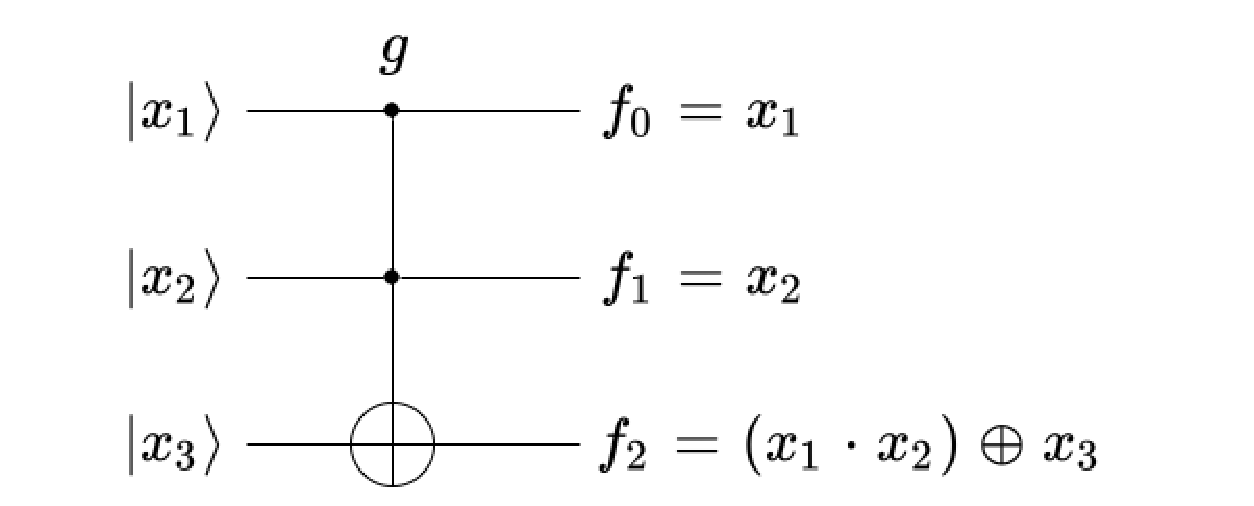
\includegraphics[width=5cm]{img/toffoli-f.eps}
    \caption{Functional representations for the output of a Toffoli gate.}
    \label{toffoli-f}
  \end{center}
  %\vspace*{-1cm}
\end{figure}
\begin{figure}[t]
  \label{fig-bool-or}
\end{figure}
\begin{figure}[t]
  \label{fig-bool-and}
\end{figure}


\section{Preliminary}
\label{Sec:prelim}
\subsection{Quantum Boolean Circuits}

In this paper, we consider {\it quantum Boolean circuits}~\cite{bib-ddmf} that implement Boolean functions, consisting of Toffoli gates, T gates, S gates and relative-phase Toffoli gates (RTOFs)~\cite{bib-rtof}. 

We denote the primary inputs of a circuit by $x_1, x_2, \cdots,x_{n}$  when we have $n$ primary inputs. Each qubit state in a circuit consisting of Toffoli and RTOF gates can be represented by a Boolean function with respect to $x_1, x_2, \cdots,x_{n}$.

 \subsection{Boolean Constructions}
 \label{Sec:bool-const}
We will be using a few common constructions to realize certain Boolean operations as quantum circuits. Fig.~\ref{fig-bool-or} depicts how putting the output of two Toffoli or CNOT gates in series on the same output qubit will create a Boolean sum of their controls, while ~\ref{fig-bool-and} depicts how putting their outputs in parallel on the controls of a Toffoli gate will produce their Boolean product on the Toffoli gate's output (assuming a clean ancilla). We will be using these facts in the next section. 

\subsection{Relative-Phase Toffoli Gates (RTOFs)}

An RTOF (Relative-Phase Toffoli) gate~\cite{bib-rtof} has two control bits and one target bit. It inverts the basis state of the target bit (i.e., $\ket{1}$ to $\ket{0}$ and $\ket{0}$ to $\ket{1}$) when the states of the both control bits are $\ket{11}$. A Toffoli gate consists of 7 T gates as shown in Fig.~\ref{toffoli} whereas an RTOF consists of 4 T gates as shown in Fig.~\ref{rtof}. One may notice that the version of the RTOF that is used here is similar to the n-controlled-iX gate from ~\cite{bib-selinger-rtof} for $n=2$, with one less CNOT gate. As noted in ~\cite{bib-rtof}, removing this gate only affects the phase, so it only transforms an RTOF gate into another RTOF gate. We will subsume this

As depicted in Fig.~\ref{rtof}, an RTOF has three inputs; the input quantum basis states are $\ket{000}$ to $\ket{111}$. Similar to Toffoli gates, an RTOF swaps  $\ket{110}$ and $\ket{111}$. In addition to this logic operation, RTOF gates add phases to some output states that the equivalent Toffoli gate does not. The added phases are as shown in Table~\ref{table-rtof}. For example, when the input state is $\ket{110}$, a phase $+\pi/2$ is added.

One of the results from ~\cite{bib-rtof} is that when larger functions are broken down into compute/uncompute pairs, such as in the Barenco style Toffoli decompositions, it is almost always more advantageous to implement each ``half'' of the compute/uncompute pair into a relative phase construction. We will next go into one such construction.

\subsection{Relative-Phase Boolean Functions}

As an extension of the RTOF

\subsection{Boolean Logic Network}

A {\it Boolean Logic Network} is a simple dag whose vertices are primary inputs, primary outputs, and nodes which represent logic gates, whose arcs connect gates to inputs, outputs, and other gates.

A node {\it n} has zero or more {\it fanins}, or incoming edges, and zero or more {\it fanouts} i.e. outgoing edges. The {\it primary inputs (PIs)} are nodes without fanins in the current network. The {\it primary outputs} are a subset of nodes of the network without fanouts. 

A logic function can be decomposed into such a Boolean Logic Network, and its nodes subsequently implemented as LUTs or logic gates.

 \section{Existing Research}
 \label{Sec:Exist}
\subsection{LUT-based Hierarchical Reversible Logic Synthesis (LHRS)}
\label{Sec:lhrs}
Previous Research ~\cite{bib-soeken2018lut} has detailed a way to leverage LUT-based synthesis of Boolean functions to create reversible logic networks that will be essential to quantum Boolean circuits. The overall flow maps each node in the Boolean Network to a function-controlled NOT gate, and then cascades them together to create the output. Because the U-controlled NOT gates act on ancillas, there is a need to uncompute them, so the flow next produces uncompute logic. This produces the compute/uncompute pair that a relative-phase based construction of the function can take advantage of. 

\subsection{Using RTOF to decompose MCT gates}
Existing research ~\cite{bib-rtof} finds an advantage to using RTOFs in synthesizing and decomposing logic functions, particularly MCTs. For the sake of brevity, we will only detail their results here that we will use.
\begin{itemize}
\item Replacing pairs of computing and uncomputing gates with RTOF and its inverse will lead to T gate savings in most cases
\item Using the above, it is possible to use clean-ancilla to decompose an MCT with fewer T gates than the known methods.
\item A recursive procedure to generate MCT gates up to a relative phase
\end{itemize}
%%% Local Variables:
%%% mode: japanese-latex
%%% TeX-master: "main"
%%% End:
